\documentclass[border=10pt]{standalone}
\usepackage{pgfplots}
\pgfplotsset{compat=1.18, trig format plots=rad}
\usepackage{tikz}
\begin{document}
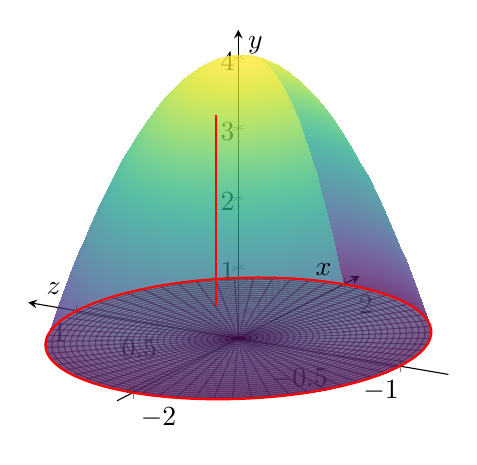
\begin{tikzpicture}
\begin{axis}[
    view={-60}{25},
    axis lines=center,
    xlabel=$x$, ylabel=$z$, zlabel=$y$,
    domain=0:1, y domain=0:2*pi,
    samples=32, samples y=64,
    xmin=-2.3, xmax=2.3, ymin=-1.3, ymax=1.3, zmin=0, zmax=4.4,
    colormap/viridis,
    width=10cm, height=8cm,
]
\addplot3[surf, opacity=0.75, shader=interp] ({2*x*cos(y)}, {x*sin(y)}, {4*(1-x^2)});
\addplot3[surf, opacity=0.25, fill=gray] ({2*x*cos(y)}, {x*sin(y)}, {0});
\addplot3[red, thick, samples=80, domain=0:2*pi] ({2*cos(x)}, {sin(x)}, {0});
\addplot3[red, thick] coordinates {(0.8,0.4,0) (0.8,0.4,2.72)};
\end{axis}
\end{tikzpicture}
\end{document}
